\documentclass{standalone}
\usepackage{tikz}
\usetikzlibrary{patterns}
\usetikzlibrary{positioning}
\usetikzlibrary{patterns, positioning}
\usetikzlibrary{shapes.misc}
\usepackage[outline]{contour}
\contourlength{1.5pt} 
\usepackage[sfdefault]{ClearSans}

\begin{document}
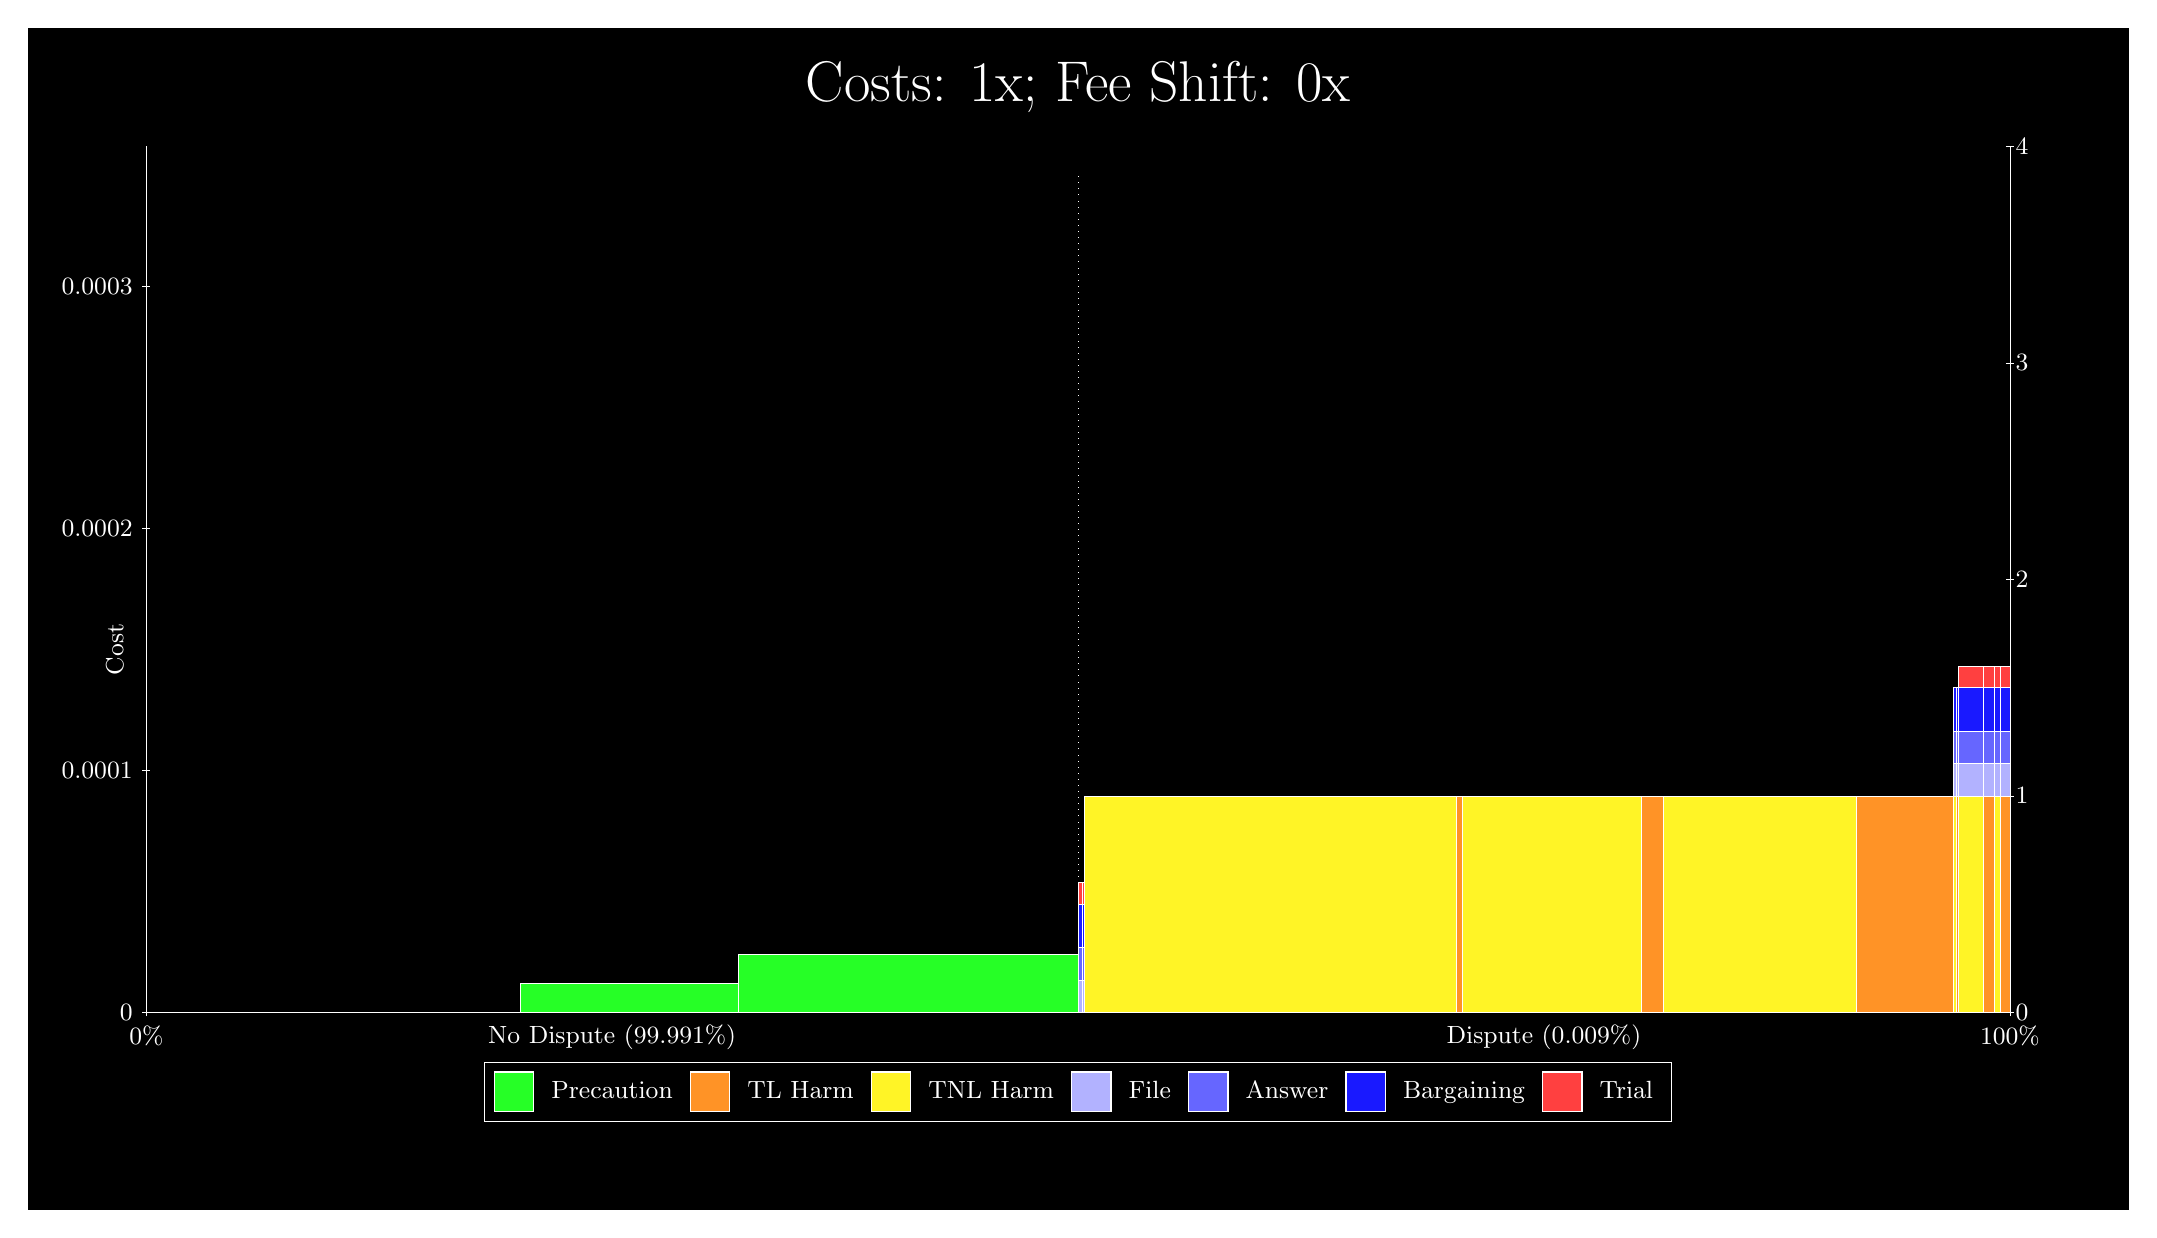
\begin{tikzpicture}
\draw[fill=black] (0,0) rectangle (26.667,15);
\draw[draw=none,text=white] (0,13.5) rectangle (26.667,15) node[midway] {\huge Costs: 1x; Fee Shift: 0x };
\draw[fill=green!85,draw=white,very thin] (6.2548,2.5) rectangle (9.0126,2.8688);
\draw[fill=green!85,draw=white,very thin] (9.0126,2.5) rectangle (13.333,3.2377);
\draw[fill=blue!30,draw=white,very thin] (13.333,2.5) rectangle (13.339,2.9125);
\draw[fill=blue!60,draw=white,very thin] (13.333,2.9125) rectangle (13.339,3.325);
\draw[fill=blue!90,draw=white,very thin] (13.333,3.325) rectangle (13.339,3.875);
\draw[fill=blue!30,draw=white,very thin] (13.339,2.5) rectangle (13.385,2.9125);
\draw[fill=blue!60,draw=white,very thin] (13.339,2.9125) rectangle (13.385,3.325);
\draw[fill=blue!90,draw=white,very thin] (13.339,3.325) rectangle (13.385,3.875);
\draw[fill=red!75,draw=white,very thin] (13.339,3.875) rectangle (13.385,4.15);
\draw[fill=green!85,draw=white,very thin] (13.385,2.5) rectangle (13.408,2.5);
\draw[fill=blue!30,draw=white,very thin] (13.385,2.5) rectangle (13.408,2.9125);
\draw[fill=blue!60,draw=white,very thin] (13.385,2.9125) rectangle (13.408,3.325);
\draw[fill=blue!90,draw=white,very thin] (13.385,3.325) rectangle (13.408,3.875);
\draw[fill=red!75,draw=white,very thin] (13.385,3.875) rectangle (13.408,4.15);
\draw[fill=yellow!85,draw=white,very thin] (13.408,2.5) rectangle (18.139,5.25);
\draw[fill=orange!85,draw=white,very thin] (18.139,2.5) rectangle (18.207,5.25);
\draw[fill=green!85,draw=white,very thin] (18.207,2.5) rectangle (20.481,2.5);
\draw[fill=yellow!85,draw=white,very thin] (18.207,2.5) rectangle (20.481,5.25);
\draw[fill=green!85,draw=white,very thin] (20.481,2.5) rectangle (20.769,2.5);
\draw[fill=orange!85,draw=white,very thin] (20.481,2.5) rectangle (20.769,5.25);
\draw[fill=green!85,draw=white,very thin] (20.769,2.5) rectangle (23.214,2.5001);
\draw[fill=yellow!85,draw=white,very thin] (20.769,2.5001) rectangle (23.214,5.2501);
\draw[fill=green!85,draw=white,very thin] (23.214,2.5) rectangle (24.45,2.5001);
\draw[fill=orange!85,draw=white,very thin] (23.214,2.5001) rectangle (24.45,5.2501);
\draw[fill=yellow!85,draw=white,very thin] (24.45,2.5) rectangle (24.488,5.25);
\draw[fill=blue!30,draw=white,very thin] (24.45,5.25) rectangle (24.488,5.6625);
\draw[fill=blue!60,draw=white,very thin] (24.45,5.6625) rectangle (24.488,6.075);
\draw[fill=blue!90,draw=white,very thin] (24.45,6.075) rectangle (24.488,6.625);
\draw[fill=orange!85,draw=white,very thin] (24.488,2.5) rectangle (24.51,5.25);
\draw[fill=blue!30,draw=white,very thin] (24.488,5.25) rectangle (24.51,5.6625);
\draw[fill=blue!60,draw=white,very thin] (24.488,5.6625) rectangle (24.51,6.075);
\draw[fill=blue!90,draw=white,very thin] (24.488,6.075) rectangle (24.51,6.625);
\draw[fill=yellow!85,draw=white,very thin] (24.51,2.5) rectangle (24.835,5.25);
\draw[fill=blue!30,draw=white,very thin] (24.51,5.25) rectangle (24.835,5.6625);
\draw[fill=blue!60,draw=white,very thin] (24.51,5.6625) rectangle (24.835,6.075);
\draw[fill=blue!90,draw=white,very thin] (24.51,6.075) rectangle (24.835,6.625);
\draw[fill=red!75,draw=white,very thin] (24.51,6.625) rectangle (24.835,6.9);
\draw[fill=orange!85,draw=white,very thin] (24.835,2.5) rectangle (24.966,5.25);
\draw[fill=blue!30,draw=white,very thin] (24.835,5.25) rectangle (24.966,5.6625);
\draw[fill=blue!60,draw=white,very thin] (24.835,5.6625) rectangle (24.966,6.075);
\draw[fill=blue!90,draw=white,very thin] (24.835,6.075) rectangle (24.966,6.625);
\draw[fill=red!75,draw=white,very thin] (24.835,6.625) rectangle (24.966,6.9);
\draw[fill=green!85,draw=white,very thin] (24.966,2.5) rectangle (25.046,2.5);
\draw[fill=yellow!85,draw=white,very thin] (24.966,2.5) rectangle (25.046,5.25);
\draw[fill=blue!30,draw=white,very thin] (24.966,5.25) rectangle (25.046,5.6625);
\draw[fill=blue!60,draw=white,very thin] (24.966,5.6625) rectangle (25.046,6.075);
\draw[fill=blue!90,draw=white,very thin] (24.966,6.075) rectangle (25.046,6.625);
\draw[fill=red!75,draw=white,very thin] (24.966,6.625) rectangle (25.046,6.9);
\draw[fill=green!85,draw=white,very thin] (25.046,2.5) rectangle (25.167,2.5);
\draw[fill=orange!85,draw=white,very thin] (25.046,2.5) rectangle (25.167,5.25);
\draw[fill=blue!30,draw=white,very thin] (25.046,5.25) rectangle (25.167,5.6625);
\draw[fill=blue!60,draw=white,very thin] (25.046,5.6625) rectangle (25.167,6.075);
\draw[fill=blue!90,draw=white,very thin] (25.046,6.075) rectangle (25.167,6.625);
\draw[fill=red!75,draw=white,very thin] (25.046,6.625) rectangle (25.167,6.9);
\draw[white,very thin] (1.5,2.5) -- (1.5,13.5);
\node[font=\small,rotate=90,text=white, anchor=center] at (1.1, 7.1104) {Cost};
\draw[white,very thin] (1.45,2.5) -- (1.55,2.5);
\node[font=\small,text=white, anchor=east] at (1.45, 2.5) {0};
\draw[white,very thin] (1.45,5.5736) -- (1.55,5.5736);
\node[font=\small,text=white, anchor=east] at (1.45, 5.5736) {0.0001};
\draw[white,very thin] (1.45,8.6472) -- (1.55,8.6472);
\node[font=\small,text=white, anchor=east] at (1.45, 8.6472) {0.0002};
\draw[white,very thin] (1.45,11.721) -- (1.55,11.721);
\node[font=\small,text=white, anchor=east] at (1.45, 11.721) {0.0003};

\draw[white,dotted,very thin] (13.333,2.83) -- (13.333,13.17);
\draw[white,very thin] (25.167,2.5) -- (25.167,13.5);
\draw[white,very thin] (25.117,2.5) -- (25.217,2.5);
\node[font=\small,text=white, anchor=west] at (25.117, 2.5) {0};
\draw[white,very thin] (25.117,5.25) -- (25.217,5.25);
\node[font=\small,text=white, anchor=west] at (25.117, 5.25) {1};
\draw[white,very thin] (25.117,8) -- (25.217,8);
\node[font=\small,text=white, anchor=west] at (25.117, 8) {2};
\draw[white,very thin] (25.117,10.75) -- (25.217,10.75);
\node[font=\small,text=white, anchor=west] at (25.117, 10.75) {3};
\draw[white,very thin] (25.117,13.5) -- (25.217,13.5);
\node[font=\small,text=white, anchor=west] at (25.117, 13.5) {4};

\draw[white,very thin] (1.5,2.5) -- (25.167,2.5);
\draw[white,very thin] (1.5,2.45) -- (1.5,2.55);
\node[font=\small,text=white, anchor=north] at (1.5, 2.45) {0\%};
\draw[white,very thin] (25.167,2.45) -- (25.167,2.55);
\node[font=\small,text=white, anchor=north] at (25.167, 2.45) {100\%};

\node[font=\small,text=white,anchor=south] at (7.4167, 1.9) {No\ Dispute\ (99.991\%)};
\node[font=\small,text=white,anchor=south] at (19.25, 1.9) {Dispute\ (0.009\%)};
\draw (13.3333,2.5) node (B) {};
\begin{scope}[align=center]
\matrix[scale=0.5,draw=white,below=0.5cm of B,nodes={draw},column sep=0.1cm]{
\node[rectangle,draw,minimum width=0.5cm,minimum height=0.5cm,fill=green!85]{}; & \node[draw=none,font=\small,text=white]{Precaution}; &
\node[rectangle,draw,minimum width=0.5cm,minimum height=0.5cm,fill=orange!85]{}; & \node[draw=none,font=\small,text=white]{TL Harm}; &
\node[rectangle,draw,minimum width=0.5cm,minimum height=0.5cm,fill=yellow!85]{}; & \node[draw=none,font=\small,text=white]{TNL Harm}; &
\node[rectangle,draw,minimum width=0.5cm,minimum height=0.5cm,fill=blue!30]{}; & \node[draw=none,font=\small,text=white]{File}; &
\node[rectangle,draw,minimum width=0.5cm,minimum height=0.5cm,fill=blue!60]{}; & \node[draw=none,font=\small,text=white]{Answer}; &
\node[rectangle,draw,minimum width=0.5cm,minimum height=0.5cm,fill=blue!90]{}; & \node[draw=none,font=\small,text=white]{Bargaining}; &
\node[rectangle,draw,minimum width=0.5cm,minimum height=0.5cm,fill=red!75]{}; & \node[draw=none,font=\small,text=white]{Trial}; \\\\
};\end{scope}

\end{tikzpicture}
\end{document}